\documentclass[border=10pt]{standalone}
\usepackage{pgfplots}
\usepackage{amsmath}
\pgfplotsset{compat=1.18}
\usepackage{xcolor}

\definecolor{mlmcolor}{RGB}{50,120,200}
\definecolor{clscolor}{RGB}{220,80,40}
\definecolor{predcolor}{RGB}{150,150,150}

\begin{document}
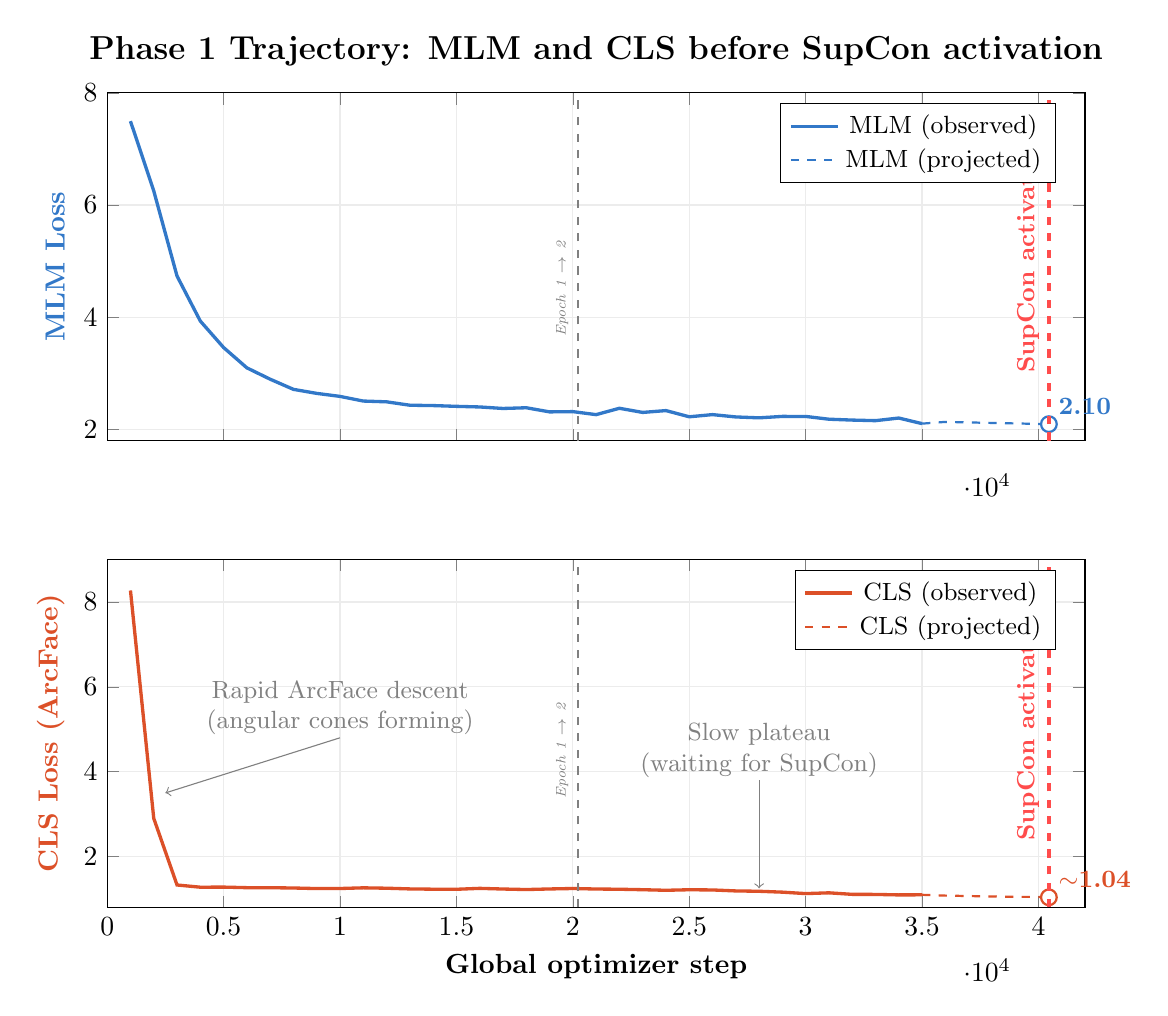
\begin{tikzpicture}

% MLM plot (top)
\begin{axis}[
  name=mlmplot,
  width=14cm, height=6cm,
  xlabel={},
  ylabel={MLM Loss},
  ylabel style={font=\bfseries, text=mlmcolor},
  xmin=0, xmax=42000,
  ymin=1.8, ymax=8,
  xtick={0,5000,10000,15000,20000,25000,30000,35000,40000},
  xticklabels={},
  grid=major,
  grid style={gray!15},
  title={\textbf{Phase 1 Trajectory: MLM and CLS before SupCon activation}},
  title style={font=\large},
  legend pos=north east,
  legend style={font=\small},
  clip=false,
]

% MLM actual data
\addplot[mlmcolor, very thick, mark=none] coordinates {
  (1000,7.4944) (2000,6.2520) (3000,4.7343) (4000,3.9321) (5000,3.4602)
  (6000,3.0982) (7000,2.8959) (8000,2.7148) (9000,2.6430) (10000,2.5894)
  (11000,2.5064) (12000,2.4927) (13000,2.4320) (14000,2.4259) (15000,2.4121)
  (16000,2.4012) (17000,2.3742) (18000,2.3870) (19000,2.3135) (20000,2.3179)
  (21000,2.2643) (22000,2.3777) (23000,2.3037) (24000,2.3365) (25000,2.2260)
  (26000,2.2648) (27000,2.2232) (28000,2.2073) (29000,2.2328) (30000,2.2324)
  (31000,2.1828) (32000,2.1673) (33000,2.1570) (34000,2.2037) (35000,2.1040)
};
\addlegendentry{MLM (observed)}

% MLM extrapolation
\addplot[mlmcolor, thick, dashed, mark=none] coordinates {
  (35000,2.1040) (36000,2.1350) (37000,2.1256) (38000,2.1165)
  (39000,2.1076) (40000,2.0990) (40448,2.095)
};
\addlegendentry{MLM (projected)}

% Predicted landing point
\node[mlmcolor, fill=white, draw=mlmcolor, thick, circle, inner sep=2pt]
  at (axis cs:40448,2.095) {};
\node[mlmcolor, font=\small\bfseries, anchor=south west]
  at (axis cs:40448,2.095) {2.10};

% Epoch boundary
\draw[gray, dashed, thick] (axis cs:20224,1.8) -- (axis cs:20224,8);
\node[font=\tiny\itshape, text=gray, rotate=90, anchor=south]
  at (axis cs:20224,4.5) {Epoch 1 $\to$ 2};

% SupCon activation line
\draw[red!70, very thick, dashed] (axis cs:40448,1.8) -- (axis cs:40448,8);
\node[font=\small\bfseries, text=red!70, rotate=90, anchor=south]
  at (axis cs:40448,5.0) {SupCon activates};

\end{axis}

% CLS plot (bottom)
\begin{axis}[
  at=(mlmplot.below south west),
  anchor=north west,
  yshift=-0.8cm,
  width=14cm, height=6cm,
  xlabel={\textbf{Global optimizer step}},
  ylabel={CLS Loss (ArcFace)},
  ylabel style={font=\bfseries, text=clscolor},
  xmin=0, xmax=42000,
  ymin=0.8, ymax=9,
  xtick={0,5000,10000,15000,20000,25000,30000,35000,40000},
  grid=major,
  grid style={gray!15},
  legend pos=north east,
  legend style={font=\small},
  clip=false,
]

% CLS actual data
\addplot[clscolor, very thick, mark=none] coordinates {
  (1000,8.2727) (2000,2.9012) (3000,1.3304) (4000,1.2783) (5000,1.2803)
  (6000,1.2672) (7000,1.2663) (8000,1.2593) (9000,1.2459) (10000,1.2475)
  (11000,1.2634) (12000,1.2543) (13000,1.2378) (14000,1.2313) (15000,1.2292)
  (16000,1.2510) (17000,1.2352) (18000,1.2230) (19000,1.2368) (20000,1.2475)
  (21000,1.2353) (22000,1.2302) (23000,1.2192) (24000,1.2055) (25000,1.2182)
  (26000,1.2133) (27000,1.1904) (28000,1.1822) (29000,1.1615) (30000,1.1275)
  (31000,1.1457) (32000,1.1098) (33000,1.1081) (34000,1.0965) (35000,1.0989)
};
\addlegendentry{CLS (observed)}

% CLS extrapolation
\addplot[clscolor, thick, dashed, mark=none] coordinates {
  (35000,1.0989) (36000,1.08) (37000,1.07) (38000,1.06)
  (39000,1.05) (40000,1.05) (40448,1.04)
};
\addlegendentry{CLS (projected)}

% Predicted landing point
\node[clscolor, fill=white, draw=clscolor, thick, circle, inner sep=2pt]
  at (axis cs:40448,1.04) {};
\node[clscolor, font=\small\bfseries, anchor=south west]
  at (axis cs:40448,1.04) {$\sim$1.04};

% Epoch boundary
\draw[gray, dashed, thick] (axis cs:20224,0.8) -- (axis cs:20224,9);
\node[font=\tiny\itshape, text=gray, rotate=90, anchor=south]
  at (axis cs:20224,4.5) {Epoch 1 $\to$ 2};

% SupCon activation line
\draw[red!70, very thick, dashed] (axis cs:40448,0.8) -- (axis cs:40448,9);
\node[font=\small\bfseries, text=red!70, rotate=90, anchor=south]
  at (axis cs:40448,5.0) {SupCon activates};

% Annotation
\node[font=\small, text=gray, align=center] at (axis cs:10000,5.5)
  {Rapid ArcFace descent\\(angular cones forming)};
\draw[gray, thin, ->] (axis cs:10000,4.8) -- (axis cs:2500,3.5);

\node[font=\small, text=gray, align=center] at (axis cs:28000,4.5)
  {Slow plateau\\(waiting for SupCon)};
\draw[gray, thin, ->] (axis cs:28000,3.8) -- (axis cs:28000,1.25);

\end{axis}

\end{tikzpicture}
\end{document}
